\chapter{Meta}

\section{Hintergrund}

Das Internet der Dinge wird Tag für Tag größer. Der Einfluss den smarte Geräte in modernen Haushälten haben wird ständig stärker. Die meisten Hersteller von smarten Geräten zielen auf Benutzerfreundlichkeit und Einfachkeit ab. Die vielen Do-It-Yourself Enthusiasten rücken für sie in den Hintergrund. Einer wichtigsten und am Häufigsten genutzten Mechanismen in einem Haushalt sind Schlösser.  Da nicht jeder der selbst gerne Sachen in die Hand nimmt die Fähigkeiten oder Zeit besitzt, ein sicheres und smartes Türschloss von Grund auf zu entwerfen und aufzubauen, haben wir uns entschieden, ein intelligentes Türschloss zu entwickeln.

\section{Namensherkunft}

Der Name \textbf{Shulker} stammt ursprünglich aus der dem Videospiel \textit{Minecraft}. In Minecraft ist ein Shulker eine Kreatur, die Verschlossen ist.

\begin{figure}[H]
    \begin{center}
        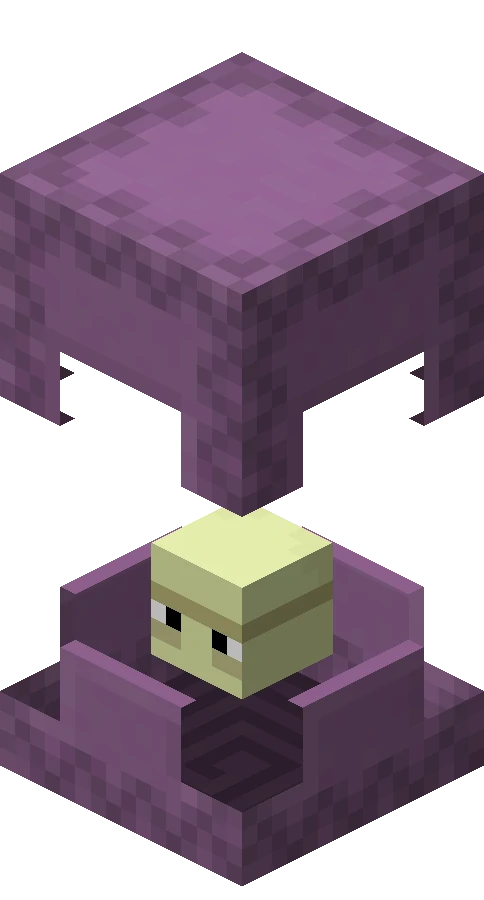
\includegraphics[width=0.22\textwidth]{images/Intro/Shulker.png}
        \caption{Die Kreatur \textbf{Shulker} aus dem Videospiel \textit{Minecraft}}
        \cite{mcwiki2015}
    \end{center}
\end{figure}

\newpage